\lstset{language=VBScript,
        basicstyle=\footnotesize\ttfamily,
        breaklines=true,
        tabsize=2,
        numbers=left,
        numberstyle=\tiny,
        numbersep=7pt,
        showspaces=false,
        keywordstyle=\color{Blue}\textbf,
        commentstyle=\color{Red}\emph,
        showstringspaces=false,
        stringstyle=\color{BurntOrange}
        }
\section{Specyfikacja wewnętrzna}
Oprogramowanie zostało stworzone w~całości Javie. Dla~ułatwienia kompilacji, zarządzanie zależnościami oraz wersjami zastosowano Apache Maven, które jest narzędziem automatyzującym budowę oprogramowania.
Najważniejszymi bibliotekami wykorzystywanymi w~projekcie są:
\begin{enumerate}
\item RXTX \newline
W~zasadzie najważniejsza biblioteka w~całym projekcie wykorzystywana do~komunikacji poprzez port szeregowy.
\item SWT: The Standard Widget Toolkit \newline
Biblioteka wykorzystana do stworzenia GUI (graficzny interfejs użytkownika) aplikacji. Dostarcza sporą ilość gotowych komponentów, które trzeba odpowiednio oprogramować. Biblioteka jest zależna od architektury i~systemu operacyjnego co~zostało uwzględnione jako profile Mavena.
\item iText \newline
Biblioteka iText służy głównie do tworzenia dokumentów PDF przez programy napisane w Javie. Jej~dodatkowe możliwości~to
obsługa formatów RTF i~HTML. Biblioteka została zastosowana do generowania raportu z~pomiaru w~formacie~PDF.
\item Apache POI \newline
Zbiór bibliotek do obsługi plików w formacie Microsoft OLE~2 z~poziomu języka programowania Java. W naszym projekcie wykorzystujemy tylko HSSF, który umożliwia obsługę plików Microsoft Excel. Biblioteka została zastosowana do generowania raportu z~pomiaru w~formacie~XLS.
\item Hibernate \newline
Framework do realizacji warstwy dostępu do danych (ang. persistance layer). Zapewnia on przede wszystkim translację danych pomiędzy relacyjną bazą danych, a światem obiektowym (ang. O/R mapping). Opiera się na wykorzystaniu opisu struktury danych za pomocą języka XML, dzięki czemu można "rzutować" obiekty, stosowane w obiektowych językach programowania, takich jak Java bezpośrednio na~istniejące tabele bazy danych.
\item dom4j \newline
dom4j to kolejny projekt typu open-source. Jego API oparte jest na interfejsach. Korzysta z parsera SAX. Jego motywacja jest podobna jak JDOM: prostsze i~lżejsze od~DOM API, stworzone specjalnie dla języka Java. W~projekcie wykorzystywany do~odczytu oraz zapisu pliku zawierającego konfigurację urządzeń oraz precyzję pomiarów.
\end{enumerate}
\newpage
Maven umożliwia stworzenie profili, które wykonują różne zadania lub pozwalają rozróżnić odrębne niezależne przebiegi kompilacji. W~naszym projekcie wykorzystaliśmy je do~pobrania i~dołączenia do~pliku końcowego biblioteki SWT w wersji dla wybranego systemu operacyjnego i~architektury. Dostępne profile Mavena:
\begin{enumerate}
\item win32 -- Windows 32-bitowy
\item win64 -- Windows 64-bitowy 
\item lin32 -- Linux 32-bitowy
\item lin64 -- Linux 64-bitowy
\item mac32 -- Mac OSX Cocoa 32-bitowy
\item mac64 -- Mac OSX Cocoa 64-bitowy
\end{enumerate}

Struktura projektu w formie diagramu:
\begin{figure}[!htb] 	
\centering 	
\begin{tikzpicture}[node distance=1.1cm]
    \node (GasAnalyzer) [abstract, rectangle split, rectangle split parts=2]
        {
            \textbf{GasAnalyzer}
            \nodepart{second}wersja 0.1.0
        };
	\node (AuxNode01) [text width=4cm, below=of GasAnalyzer] {};
    \node (ELANNetwork) [abstract, rectangle split, rectangle split parts=2, left=of AuxNode01]
        {
            \textbf{ELANNetwork}
            \nodepart{second}wersja 0.1.0
        };
    \node (GasAnalyzerGUI) [abstract, rectangle split, rectangle split parts=2, right=of AuxNode01]
        {
            \textbf{GasAnalyzerGUI}
            \nodepart{second}wersja 0.1.0
        };    
    \draw[myarrow] (ELANNetwork.north) -- ++(0,0.1) -| (GasAnalyzer.south);
    \draw[line] (ELANNetwork.north) -- ++(0,0.1) -| (GasAnalyzerGUI.north); 
        
\end{tikzpicture}
\caption{Struktura projektu} 
\label{projectSchema}
 \end{figure}

\subsection{Baza danych}
W~programie wykorzystujemy bazę PostgreSQL. Do obsługi w~aplikacji wykorzystujemy omówioną już wcześniej bibliotekę Hibernate. Schemat bazy danych został stworzony w~pgDesignerze i~wygląda jak na Rysunku~\ref{databaseSchema}.
\begin{figure}[!htb] 	
\centering 	
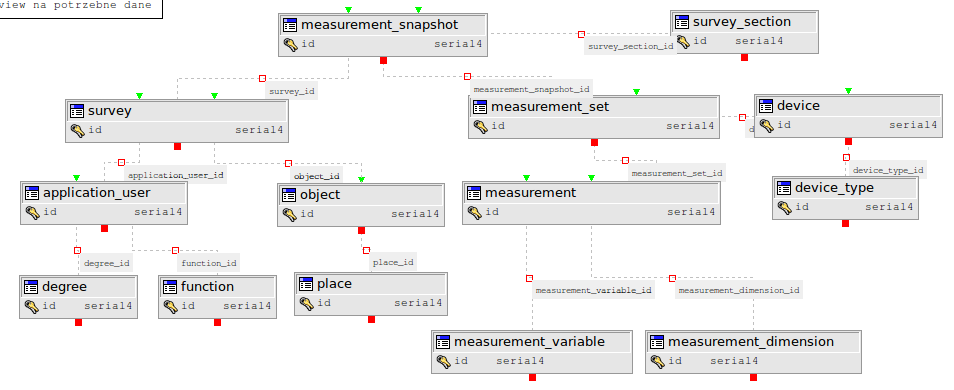
\includegraphics[width=0.9\textwidth]{images/database} 
\caption{Schemat bazy danych} 
\label{databaseSchema}
 \end{figure}